\section{Cactus Environment Calculus} \label{sec:calc}

This section shows how the shared environment approach can be applied to
call-by-need evaluation. We start with a calculus that abstracts away
environment representation, Curien's calculus of closures, and we show how it
can be modified to force sharing. See Curien's call-by-name calculus of closures
in Figure~\ref{fig:calcclos}. \footnote{Curien calls it a ``lazy'' evaluator, and
there is some ambiguity with the term lazy, but we use the term only to mean
call-by-need. We also remove the condition checking that $i < m$ because we are
only concerned with evaluation of closed terms.}

The LEval rule pushes a closure onto the environment, and the LVar rule indexes
into the environment, entering the corresponding closure. We show in this
section that by removing ambiguity about how the environments are represented,
and forcing them to be represented in a \emph{cactus stack}
~\cite{stenstrom1988vlsi}, we can define our novel call-by-need calculus.

To start, consider again the example from Section~\ref{sec:env}, this
time with deBruijn indices: $(\lambda(\lambda t) \; (\lambda t_1)) t_2$.  The
terms $t$ and $t_1$, when evaluated in the closure calculus, would have the
following environments, respectively: 

\begin{center}
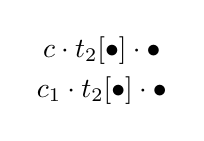
\begin{tikzpicture}
\node {$c \cdot t_2[\bullet] \cdot \bullet$};
\node [yshift=-0.5cm] {$c_1 \cdot t_2[\bullet] \cdot \bullet$};
\end{tikzpicture}
\end{center}

Again, the second closure is identical in each environment.  And again,
we can represent these environments with a shared environment, this time
keeping call-by-need evaluation in mind:
\begin{center}
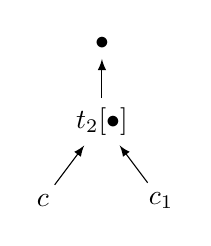
\begin{tikzpicture}[ 
  edge from parent path={(\tikzchildnode\tikzchildanchor) edge [-latex] (\tikzparentnode\tikzparentanchor)},
  level distance=1cm
]
\node (a) {$\bullet$} child{node (d) {$t_2[\bullet]$} child{node (b) {$c$}} child{node (c)
{$c_1$}}};

%\draw let \p1=(a), \p2 =(b), \n1={atan2(\y2-\y1,\x2-\x1)}, \n2={veclen(\y2-\y1,\x2-\x1)}
%  in ($ (a)!0.5!(b) $) ellipse [x radius=\n2/2+10pt, y radius=10pt, rotate=90-\n1];
%\draw let \p1=(a), \p2 =(c), \n1={atan2(\y2-\y1,\x2-\x1)}, \n2={veclen(\y2-\y1,\x2-\x1)}
%  in ($ (a)!0.5!(c) $) ellipse [x radius=\n2/2+10pt, y radius=10pt, rotate=90-\n1];
\end{tikzpicture}
\end{center}
This inverted tree structure seen earlier with the leaves pointing toward the
root is called a \emph{cactus stack} (sometimes called a spaghetti stack or
saguaro stack) \cite{hauck1968burroughs,ichbiah1991rationale}. In this
particular cactus stack, every node defines an environment as the sequence of
closures in the path to the root.  If $t_2[\bullet]$ is a thunk, and is updated
in place with the value after its first reference, then both environments would
contain the resulting value. This is exactly the kind of sharing that is
required by call-by-need, and thus we can use this structure to build a
call-by-need evaluator. This is the essence of the cactus environment calculus
and the cactus environment ($\mathcal{\mathcal{C} \mskip -4mu \mathcal{E}}$) machine. 

Curien's calculus of closures does not differentiate between flat and shared
environment representations, and indeed, no calculus that we are aware of has
had the need to. Therefore, we must derive a calculus of closures, forcing the
environment to be shared. Because we can hold the closure directly in the
environment, we choose to replace the standard heap of closures with a
\emph{heap of environments}. To enforce sharing, we extend Curien's
calculus of closures to explicity include the heap of environments, which we
refer to as a \emph{cactus environment}. 

See Figure~\ref{fig:calccact} for the syntax and semantics of the cactus
calculus. Recall that we are only concerned with evaluation of closed terms. The
initial closed term $t$ is placed in a $(t[0],\epsilon[0 \mapsto \bullet])$
tuple, and evaluation terminates on a value. We use some shorthand to make heap
notation more palatable, for both the big-step semantics presented here and the
small step semantics presented in the next section. $\mu(l,i)=l' \mapsto c
\cdot l''$ denotes that looking up the $i$'th element in the linked environment
structure starting at $l$ results in location $l'$, where closure $c$ and
continuing environment $l''$ reside. $\mu(l) = c \cdot l'$ is the statement
that $l \mapsto c \cdot l' \in \mu$. $\mu(u \mapsto c \cdot l')$ is $\mu$ with
location $u$ updated to map to $c \cdot e$. $\textnormal{dom}(\mu)$ denotes the
domain of the heap $\mu$. We define two different semantics, one for call-by-name and
one for call-by-need, which makes the connection to Curien's call-by-name
calculus more straightfoward. The rule for application (MEval and NEval) is
identical for both semantics: each evaluates the left hand side to a function,
then binds the variable in the cactus environment, extending the current
environment.

The only difference between this semantics and Curien's is that if we need
to extend an environment multiple times, the semantics \emph{requires}
sharing it among the extensions. This makes no real difference for call-by-name,
but it is needed for the sharing of results in the NVar rule. The explicit
environment sharing ensures that the closure that is overwritten with a value is
shared correctly.

\begin{figure*}
\textbf{Syntax}
\begin{align*}
\tag{Term} t &::= i \; | \; \lambda t \; | \; t \; t  \\
\tag{Variable} i &\in \mathbb{N}  \\
\tag{Closure} c &::= t [l] \\
\tag{Value} v &::= \lambda t [l] \\
\tag{Heap} \mu &::= \epsilon \; | \; \mu [ l \mapsto \rho ] \\
\tag{Environment} \rho &::= \bullet \; | \; c \cdot l \\
\tag{Location} l,f &\in \mathbb{N}  \\
\tag{State} s &::= (c, \mu)
\end{align*}
\textbf{Call-by-Name Semantics}
\begin{align*}
\tag{MEval} \inference
{(t[l], \mu) \xrightarrow{* }_{M} (\lambda t_2[l'], \mu') \quad f \not \in \textnormal{dom}(\mu')}
{(t \; t_3[l], \mu) \rightarrow_{M} (t_2[f], \mu'[f \mapsto t_3[l] \cdot l'])}  
\end{align*}
\begin{align*}
\tag{MVar} \inference 
{\mu(l, i) = l' \mapsto c \cdot l''}
{(i[l],\mu) \rightarrow_M (c,\mu)}
\end{align*}
\textbf{Call-by-Need Semantics}
\begin{align*}
\tag{NEval} \inference
{(t[l], \mu) \xrightarrow{* }_{N} (\lambda t_2[l'], \mu') \quad f \not \in \textnormal{dom}(\mu')}
{(t \; t_3[l], \mu) \rightarrow_{N} (t_2[f], \mu'[f \mapsto t_3[l] \cdot l'])}  
\end{align*}
\begin{align*}
\tag{NVar} \inference
{\mu(l, i) = l' \mapsto c \cdot l'' \quad (c, \mu) \xrightarrow{* }_{N} (v, \mu')}
{(i[l],\mu) \rightarrow_N (v, \mu'(l' \mapsto v \cdot l''))}
\end{align*}
\caption{Cactus calculus syntax and semantics.}
\label{fig:calccact}
\end{figure*}

\subsection{Correctness}

Ariola et al. define the standard call-by-need semantics in
~\cite{ariola1995call}. To show correctness, we show that there is a strong
bisimulation between $\rightarrow_{N}$ and their operational
semantics, $\Downarrow$ (Figure~\ref{fig:cbn}).  

\begin{figure}
\begin{align*}
\tag{Heap} \Phi, \Psi, \Upsilon &::= x_1 \mapsto t_1, \dots, x_n \mapsto t_n
\end{align*}
\begin{align*}
\tag{Id} \inference
{\langle \Phi \rangle t \Downarrow \langle \Psi \rangle \lambda x.t'}
{\langle \Phi, x \mapsto t, \Upsilon \rangle x \Downarrow \langle \Psi, x
\mapsto \lambda x.t', \Upsilon \rangle \lambda x.t'}
\end{align*}
\begin{align*}
\tag{Abs} \inference 
{}
{\langle \Phi \rangle \lambda x . t \Downarrow \langle \Phi \rangle \lambda x.t}
\end{align*}
\begin{align*}
\tag{App} \inference
{\langle \Phi \rangle t_l \Downarrow \langle \Psi \rangle \lambda 
x.t_n \\ \langle \Psi, x' \mapsto t_m \rangle [x'/x]t_n \Downarrow \langle
\Upsilon \rangle \lambda y.t'}
{\langle \Phi \rangle t_l \; t_m \Downarrow \langle \Upsilon \rangle \lambda y.t'}
\end{align*}
\caption{Ariola et. al's Operational Semantics}
\label{fig:cbn}
\end{figure}

{\theorem \textnormal{(Strong Bisimulation)} $$\xrightarrow{}_{N} \; \sim \;
\Downarrow$$}
We start with a \emph{flattening} relation between a configuration for
$\Downarrow$ and a configuration for $\xrightarrow{}_{N}$. The deBruijn indexed
terms and the standard terms are both converted to terms that use deBruijn
indices for local variables and direct heap locations for free variables. The
flattening relation holds only when both terms are closed under their
corresponding heaps. It holds trivially for the special case of initializing
each configuration with a standard term and its corresponding deBruijn-indexed
term, respectively. The proof proceeds by induction on the step relation for
each direction of the bisimulation.

